\documentclass[10pt]{article}
\usepackage[utf8]{inputenc}
\usepackage{amsmath,amssymb}
\usepackage{multicol}
\usepackage[a4paper, total={8in, 11.3in}]{geometry}
\usepackage{blindtext}
\usepackage{graphicx}
\graphicspath{ {./images/} }
\pagenumbering{gobble}
\parindent=0pt
\newcommand{\C}{{\mathbb C}}
\newcommand{\N}{{\mathbb N}}
\newcommand{\R}{{\mathbb R}}
\newcommand{\Z}{{\mathbb Z}}
\newcommand{\ep}{\varepsilon}

\begin{document}

\begin{multicols}{3}

\textbf{Trig Sum/Difference}
\[\sin(x\pm y)=\sin x \cos y \pm \cos x \sin y\]
\[\cos(x\pm y)=\cos x \cos y \mp \sin x \sin y\]
\[\tan(x\pm y)=\frac{\tan x \pm \tan y}{1 \mp \tan x \tan y}\]
\textbf{Derivatives} 
\[\frac{d}{dx} (\tan x)=\sec^2 x\]
\[\frac{d}{dx} (\csc x)=-\csc x \cot x\]
\[\frac{d}{dx} (\sec x)=\sec x \tan x\]
\[\frac{d}{dx} (\cot x)=-\sec^2 x\]
\[\frac{d}{dx} (\arcsin x)=\frac{1}{\sqrt{1-x^2}}\]
\[\frac{d}{dx} (\arccos x)=-\frac{1}{\sqrt{1-x^2}}\]
\[\frac{d}{dx} (\arctan x)=\frac{1}{1+x^2}\]
\[\frac{d}{dx} \log |x| = \frac{1}{x}\]
\[\frac{d}{dx} b^x = b^x \log b\]
\[\frac{d}{dx} \log_b x=\frac{1}{x\log b}\]
\textbf{Limits}
\[\lim_{x\to 0}\frac{\sin x}{x}=1\]
\[\lim_{x\to 0}\frac{\cos x - 1}{x}=0\]
\textbf{Intermediate Value Theorem} \\
Suppose that $f(x)$ is continuous on the closed interval $[a,b]$. Then for any number $Y$ between $f(a)$ and $f(b)$, there exists some number $c\in [a,b]$ such that $f(c)=Y$. \\
\textbf{Definition of the Derivative} 
\[f'(a)=\lim_{h\to 0}\frac{f(a+h)-f(a)}{h}\]
\textbf{Squeeze Theorem} \\
Let $l(x),f(x),u(x)$ be functions that satisfy $l(x)\le f(x)\le u(x)$ near $x=a$. If $\lim_{x\to a}l(x)=L$ and $\lim_{x\to a}u(x)=L$, then $\lim_{x\to a}f(x)=L$. \\
\textbf{Logarithmic Differentiation}
\[\frac{f'(x)}{f(x)}=\frac{d}{dx}(\log |f(x)|)\]
\textbf{Extreme Value Theorem} \\
If $f(x)$ is continuous on the closed interval $[a,b]$, then $f(x)$ is bounded on $[a,b]$. \\
\textbf{Summation Notation} 
\[P(x)=\sum_{k=0}^d a_kx^k\]
\textbf{Related Rates} \\
Write equivalence and differentiate w.r.t. $t$. \\
\textbf{Percentage Rate of Change}
\[K(t)=\frac{f'(t)}{f(t)}\]
\textbf{Exponential Decay}
\[Q'(t)=-kQ(t)\]
\[Q(t)=Q(0)e^{-kt}\]
\[\text{Half life }=\frac{\log 2}{k}\]
\textbf{Newton's Law of Cooling}
\[T'(t)=K(T(t)-A)\]
\[T(t)=(T(0)-A)e^{kt}+A\]
\textbf{Population Growth}
\[P'(t)=bP(t)\]
\[P(t)=P_0 e^{bt}\]
\textbf{Logistic Growth}
\[P'(t)=b\Big(1-\frac{P(t)}{K}\Big)P(t)\]
\[P(t)=\frac{KP_0e^{bt}}{K-P_0+P_0e^{bt}}\]
\textbf{Mean Value Theorem} \\
If $f(x)$ is continuous on $[a,b]$ and differentiable on $(a,b)$, then there exists some number $c\in(a,b)$ such that $f'(c)=\frac{f(b)-f(a)}{b-a}$. \\
\textbf{Triangle Inequality} \\
\[|x+y|\le |x|+|y|\]
\textbf{Equal Derivatives Fact} \\
If $f'(x)=g'(x)$ on $(a,b)$, then $f(x)$ and $g(x)$ differ by a constant on $(a,b)$. \\
\textbf{Taylor Polynomials} 
\[T_n(x)=\sum_{k=0}^n \frac{1}{k!}f^{(k)}(a)(x-a)^k\]
\[T_1(x)=f(a)+f'(a)(x-a)\]
\textbf{Lagrange Remainder Formula} \\
Let $n\in \N$. If $f(x)$ is $(n+1)$-times differentiable, then there exists $c$ between $a$ and $x$ such that 
\begin{align*}
    R_n(x)&=f(x)-T_n(x)\\
    &=\frac{1}{(n+1)!}f^{(n+1)}(c)(x-a)^{n+1}
\end{align*}
If $|f^{(n+1)}(c)|\le M$ for all $c$ between $a$ and $x$, then 
\begin{align*}
    |R_n(x)|&=|f(x)-T_n(x)| \\
    &\le \frac{M}{(n+1)!}|x-a|^{n+1}
\end{align*}
\textbf{Generalized Mean Value Theorem} \\
Let $F(x)$ and $G(x)$ be continuous on $[a,b]$ and differentiable on $(a,b)$. Then there exists $c\in(a,b)$ such that $\frac{F'(c)}{G'(c)}=\frac{F(b)-F(a)}{G(b)-G(a)}$.
\textbf{First Derivative Test} \\
Let $x=c$ be a critical or singular point.
\begin{itemize}
    \item If $f'(x)>0$ to the left and $f'(x)<0$ to the right, then $f(x)$ has a local maximum at $x=c$.
    \item If $f'(x)>0$ to the right and $f'(x)<0$ to the left, then $f(x)$ has a local minimum at $x=c$.
    \item If $f'(x)$ has the same sign to the left and to the right, then $f(x)$ does not have a local extremum at $x=c$.
\end{itemize}
\textbf{Inference}
\begin{itemize}
    \item If $f'(x)<0$ for all $x<c$ and $f'(x)>0$ for all $x>c$, then $f(x)$ has its global minimum at $x=c$.
\end{itemize}
\textbf{Second Derivative Test} 
\begin{itemize}
    \item If $f'(c)=0$ and $f''(c)>0$, then $f(x)$ has a local minimum at $x=c$.
    \item If $f'(c)=0$ and $f''(c)<0$, then $f(x)$ has a local maximum at $x=c$.
\end{itemize}
\textbf{Newton's Method}
\[x_{n+1}=x_n-\frac{f(x_n)}{f'(x_n)}\]
\textbf{Convexity} \\
$f(x)$ is convex on $[A,B]$ if, for any $a,b\in\R$ such that $A\le a \le b \le B$, and for every $0<t<1$, we have 
\[(1-t)f(a)+tf(b)\ge f((1-t)a+tb)\]
Equivalent statements for twice-differentiable functions:
\begin{itemize}
    \item $f''(x) \ge 0$ 
    \item $f'(x)$ is increasing
    \item If $c\in (A,B)$ and $l(x)$ is the tangent line approximation to $f(x)$ at $x=c$, then $f(x)\ge l(x)$ for all $x\in [A,B]$. 
\end{itemize}
\textbf{Curve Sketching} 
\begin{itemize}
    \item $f(x)$: domain, asymptotes, symmetries, intercepts, positive/negative
    \item $f'(x)$: critical and singular points, local extrema, vertical tangent lines, increasing/decreasing
    \item $f''(x)$: convex/concave, inflection points
\end{itemize}
\textbf{Indeterminate Forms}
\[\frac{0}{0}, \frac{\infty}{\infty},  0\times\infty, \infty-\infty, 1^\infty, 0^0, \infty^0\]
\textbf{L'Hopital's Rule} \\
For $\frac{0}{0}$ and $\frac{\infty}{\infty}$ indeterminate forms,
\[\lim_{x\to *}\frac{f(x)}{g(x)}=\lim_{x\to *}\frac{f'(x)}{g'(x)}\]
\textbf{Polynomial Indeterminate Case}
\[\lim_{x\to\infty}(\sqrt[d]{P(x)}-x)=\frac{c_1}{d}\]
\end{multicols}

\newpage
\begin{multicols}{2}
\textbf{Exponentiation Limit Law} \\
If $\lim_{x\to *}f(x)=F$ with $F>0$ and $\lim_{x\to *}g(x)=G$, then $\lim_{x\to *}(f(x)^{g(x)})=F^G$. \\
\textbf{Composition with Exponential Limit Law} 
\begin{itemize}
    \item If $\lim_{x\to *}g(x)=G$, then $\lim_{x\to *}(e^{g(x)})=e^G$
    \item If $\lim_{x\to *}g(x)=\infty$, then $\lim_{x\to *}(e^{g(x)})=\infty$
    \item If $\lim_{x\to *}g(x)=-\infty$, then $\lim_{x\to *}(e^{g(x)})=0$
\end{itemize}
\textbf{Composition with Logarithm Limit Law}
\begin{itemize}
    \item If $\lim_{x\to *}f(x)=F$, then $\lim_{x\to *}(\log f(x))=\log F$
    \item If $\lim_{x\to *}f(x)=\infty$, then $\lim_{x\to *}(\log f(x))=\infty$
    \item If $\lim_{x\to *}f(x)=0$ and $f(x)>0$ near $x=*$, then $\lim_{x\to *}(\log f(x))=-\infty$
\end{itemize}
\end{multicols}

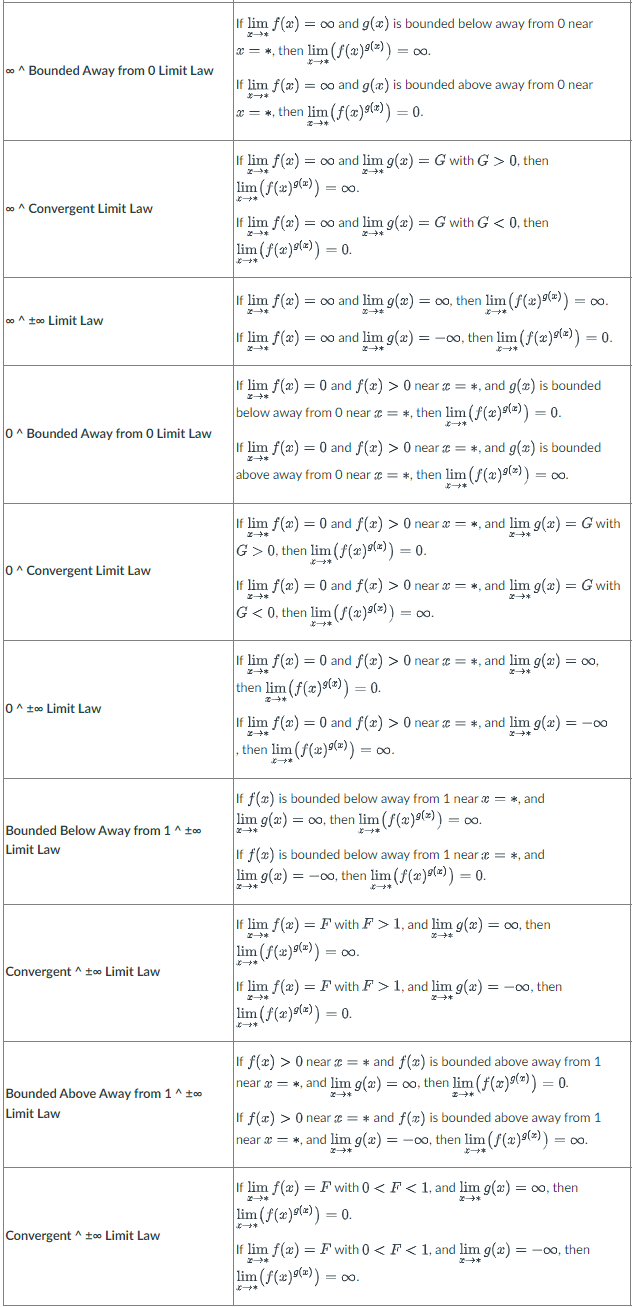
\includegraphics[scale=0.72]{exponential_limit_laws.png}


\end{document}